\documentclass{sprawozdanie-agh}

\usepackage[utf8]{inputenc}
\usepackage{matlab-prettifier}
\usepackage{siunitx}
\usepackage{svg}
\svgsetup{inkscapelatex=false}

\makeatletter

% ========= Początek Dokumentu ========= 

\begin{document}


% ========= Strona tytułowa ========= 
\przedmiot{Teoria Sterowania II: Ćwiczenia Laboratoryjne}
\tytul{Sprawozdanie: Ćwiczenie 0. }
\podtytul{Temat Demo}
\kierunek{Automatyke i Robotyka}
\autor{Dariusz Cieślar}
\data{Kraków, 27 lutego 2023}

\stronatytulowa{}

% ========= Treść Właściwa =========

\section{Cel ćwiczenia}
Krótki wstęp o czym było ćwiczenie
\section{Przebieg ćwiczenia}
Opis wykonanej pracy i rezultatów wyczerpujących opis wykonania ćwiczenia zgodnie z instrukcją
\section{Opis wniosków i obserwacji}
Kreatywne wnioski i obserwacje, które przykuły uwagę

\newpage

\section{Sekcja}
W tej sekcji kilka przykładów jak wstawiać obiekty.
\subsection{Podsekcja z tabelką}

    W tej podsekcji pokażę tabelkę.
    
    Przykładowa tabelka z odnośnikiem Tabela \ref{eq:rowstanu}
    
    \begin{table}[h!]
        \centering
        \caption{Przykład tabeli.}\label{tab1}
        \begin{tabular}{|c|c|}
            \hline
            Pora Roku &  Pierwszy dzień\\
            \hline
            Wiosna &  21 marca \\
            lato &  22 czerwca\\
            jesień & 23 września \\
            zima & 22 grudnia\\
            \hline
        \end{tabular}
    \end{table}

    

    \begin{table}[h!]
    \begin{center}
    \begin{tabular}{ c | c | c }
		 Element & Wartość & Jednostka \\ 
		 \hline\hline
		 $k_1$ & 6 & $\frac{\qty[per-mode = symbol]{}{\newton }}{\qty[per-mode = symbol]{}{\meter }}$ \\ 
		 \hline
		 $k_2$ & 2 & $\frac{\qty[per-mode = symbol]{}{\newton }}{\qty[per-mode = symbol]{}{\meter }}$ \\ 
		 \hline
		 $M$ & $1$ & $\qty[per-mode = symbol]{}{\kilogram}$ \\
		 \hline
		 $C$ & $6$ & $\frac{\qty[per-mode = symbol]{}{\newton }\qty[per-mode = symbol]{}{\second }}{\qty[per-mode = symbol]{}{\meter }}$ \\
    \end{tabular}
    \caption{Drugi przykład tabelki (kiepski).}\label{tab2}
    \end{center}
    \end{table}
    
    

\subsection{Podsekcja z równaniem i rysunkiem}
    Przykładowe równanie z odnośnikiem Równanie \ref{eq:rowstanu}
    
    \begin{equation}
    x + y = z
    \label{eq:rowstanu}
    \end{equation}

    \begin{equation} 
    \label{eqn_state2}
        \begin{bmatrix} 
            \dot{x}_1 \\  \dot{x}_2 
        \end{bmatrix} = 
        \begin{bmatrix} 0 && 1 \\ 
                        -8 && -6
        \end{bmatrix}
        \begin{bmatrix} 
            {x}_1 \\  {x}_2 
        \end{bmatrix} +
        \begin{bmatrix} 
            0 \\  1 
        \end{bmatrix} u
    \end{equation}

Przykład transmitacji $G(s)$.
        \begin{equation} 
            G(s) = \frac{1}{s^2+4s+3}
	\end{equation}

 Przykład warunków początkowych:
    \begin{equation} 
        \begin{bmatrix} 
            {x}_1 \\ {x}_2 
        \end{bmatrix} = 
        \begin{bmatrix} 0 \\ 
                        0 
        \end{bmatrix}
    \end{equation}

Przykładowy rysunek (kiepski) z odnośnikiem Rys \ref{fig1}.

    \begin{figure}[h]
    \centering
        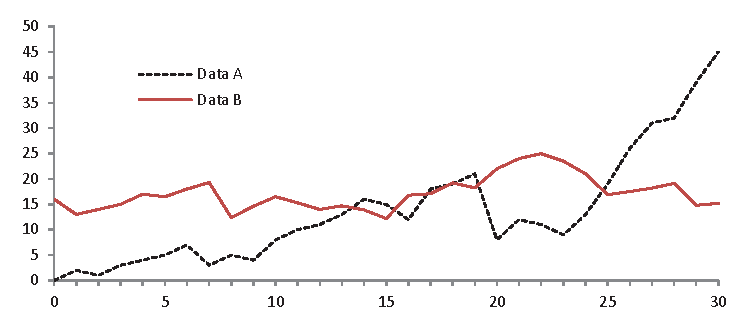
\includegraphics[width=0.2\textwidth]{fig1.eps}
        \caption{Rysunek o dwóch liniach. Na czerwono linia z danymi A, przerywaną czarną linią zilustrowano dane B.} \label{fig1}
    \end{figure}

    \begin{figure}[h!]
        \centering
        \includesvg[width=12cm]{images/SchematBlokowySprzezenie.svg}
        \caption{Schemat sprzężenia od stanu. Grafika wektorowa.}
        \label{figtest}
    \end{figure}

    \begin{figure}[h!]
        \centering
        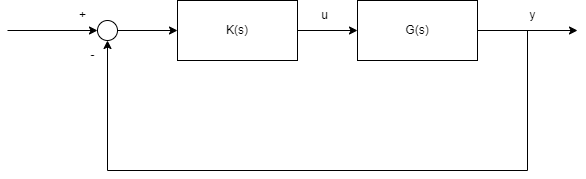
\includegraphics[width=12cm]{images/ClosedLoop.png}
        \caption{Schemat układu zamkniętego. Bitmapa.}
        \label{figtest}
    \end{figure}

I jeszcze przykładowy listing kodu z MATLABa:
    \begin{lstlisting}
        C:\Program Files\MiKTeX 2.9\tex\latex\AGH
    \end{lstlisting}

\section{Sekcja z odnośnikami}

N jeden artykuł \cite{ref_article1}


% ========= Referencje =========

\begin{thebibliography}{8}
\bibitem{ref_article1}
Author, F.: Article title. Journal \textbf{2}(5), 99--110 (2016)
\end{thebibliography}

% ========= Koniec Dokumentu =========

\end{document}